% ============================================================
%  BÁO CÁO ĐỒ ÁN TỐT NGHIỆP
%  Trường Đại học Hàng Hải Việt Nam
%  Compile: XeLaTeX (chạy 2 lần để mục lục đúng)
% ============================================================

\documentclass[13pt, a4paper]{extreport}

% ---------- Font & ngôn ngữ ----------
\usepackage{fontspec}
\setmainfont{Times New Roman}
\usepackage{polyglossia}
\setmainlanguage{vietnamese}
\setotherlanguage{english}

% ---------- Căn lề ----------
\usepackage{geometry}
\geometry{
  a4paper,
  top    = 2.0cm,
  bottom = 2.0cm,
  left   = 3.0cm,
  right  = 2.0cm
}

% ---------- Giãn dòng ----------
\usepackage{setspace}
\setstretch{1.4}

% ---------- Đoạn văn ----------
\usepackage{indentfirst}
\setlength{\parindent}{1.27cm}
\setlength{\parskip}{4pt plus 1pt minus 1pt}

% ---------- Header / Footer ----------
\usepackage{fancyhdr}
\pagestyle{fancy}
\fancyhf{}
\fancyfoot[C]{\thepage}
\renewcommand{\headrulewidth}{0pt}
\renewcommand{\footrulewidth}{0pt}

% Áp dụng cùng style cho trang đầu mỗi chương (plain)
\fancypagestyle{plain}{%
  \fancyhf{}%
  \fancyfoot[C]{\thepage}%
  \renewcommand{\headrulewidth}{0pt}%
  \renewcommand{\footrulewidth}{0pt}%
}

% ---------- Tiêu đề chương / mục ----------
\usepackage{titlesec}

% CHƯƠNG: In hoa, đậm, 17pt, căn giữa, label và tiêu đề cùng dòng
\titleformat{\chapter}[block]
  {\centering\bfseries\fontsize{17}{22}\selectfont}
  {CHƯƠNG~\thechapter:}
  {0.6em}
  {\MakeUppercase}
\titlespacing*{\chapter}{0pt}{-12pt}{18pt}

% Mục 1.1: đậm, 14pt, căn trái
\titleformat{\section}
  {\bfseries\fontsize{14}{18}\selectfont}
  {\thesection.}
  {0.6em}
  {}
\titlespacing*{\section}{0pt}{14pt}{6pt}

% Mục 1.1.1: đậm nghiêng, 13pt, căn trái
\titleformat{\subsection}
  {\bfseries\itshape\fontsize{13}{17}\selectfont}
  {\thesubsection.}
  {0.6em}
  {}
\titlespacing*{\subsection}{0pt}{10pt}{4pt}

% ---------- Mục lục ----------
\usepackage{tocloft}
\renewcommand{\cftchappresnum}{Chương~}
\renewcommand{\cftchapaftersnum}{:}
\setlength{\cftchapnumwidth}{6.5em}
\setlength{\cftsecnumwidth}{2.8em}
\setlength{\cftsubsecnumwidth}{3.8em}
\renewcommand{\cftchapleader}{\cftdotfill{\cftdotsep}}
\renewcommand{\cftsecleader}{\cftdotfill{\cftdotsep}}
\setlength{\cftbeforechapskip}{6pt}

% ---------- Bảng biểu & Hình ảnh ----------
\usepackage{graphicx}
\usepackage{float}
\usepackage{booktabs}
\usepackage{longtable}
\usepackage{array}
\usepackage{tabularx}
\usepackage{caption}
\captionsetup[table]{
  name       = Bảng,
  labelsep   = colon,
  position   = above,
  font       = {small, bf},
  justification = raggedright,
  singlelinecheck = false
}
\captionsetup[figure]{
  name       = Hình,
  labelsep   = colon,
  position   = below,
  font       = {small},
  justification = centering
}

% ---------- Danh sách ----------
\usepackage{enumitem}
\setlist[itemize]{
  leftmargin = 1.5cm,
  itemsep    = 1pt,
  topsep     = 4pt,
  parsep     = 0pt
}
\setlist[enumerate]{
  leftmargin = 1.5cm,
  itemsep    = 1pt,
  topsep     = 4pt,
  parsep     = 0pt
}

% ---------- Màu sắc & liên kết ----------
\usepackage[dvipsnames]{xcolor}
\usepackage[
  colorlinks = true,
  linkcolor  = black,
  urlcolor   = blue,
  citecolor  = black,
  pdfencoding = auto
]{hyperref}

% ---------- Miscellaneous ----------
\usepackage{amsmath}
\usepackage{rotating}   % sidewaysfigure
\usepackage{pdflscape}  % landscape page

% Đường dẫn ảnh
\graphicspath{{uml/}}

% ============================================================
\begin{document}

% ===========================================================
%  TRANG BÌA
% ===========================================================
\begin{titlepage}
  \centering
  \setstretch{1.3}

  \textbf{\large BỘ GIAO THÔNG VẬN TẢI}\\[3pt]
  \textbf{\large TRƯỜNG ĐẠI HỌC HÀNG HẢI VIỆT NAM}\\[3pt]
  \textbf{\large KHOA CÔNG NGHỆ THÔNG TIN}

  \vspace{2.2cm}

  {\fontsize{22}{28}\selectfont\bfseries BÁO CÁO ĐỒ ÁN}\\[6pt]
  {\fontsize{16}{22}\selectfont\bfseries PHÂN TÍCH VÀ THIẾT KẾ HƯỚNG ĐỐI TƯỢNG}

  \vspace{1.4cm}
  \rule{\linewidth}{1.5pt}\\[10pt]
  {\fontsize{16}{22}\selectfont\bfseries
    HỆ THỐNG GAME BATTLESHIP\\[6pt]
    TRỰC TUYẾN NHIỀU NGƯỜI CHƠI
  }\\[10pt]
  \rule{\linewidth}{1.5pt}

  \vspace{2.2cm}

  \begin{tabular}{@{}ll}
    \textbf{Môn học:}                 & Phân tích và Thiết kế Hướng Đối tượng \\[5pt]
    \textbf{Nhóm thực hiện:}          & *(Điền tên thành viên)* \\[5pt]
    \textbf{Giảng viên hướng dẫn:}    & *(Điền tên giảng viên)* \\[5pt]
    \textbf{Ngày hoàn thành:}         & Tháng 4 năm 2026 \\
  \end{tabular}

  \vfill
  {\large\bfseries Hải Phòng, 2026}
\end{titlepage}

% ===========================================================
%  MỤC LỤC  — đánh số La Mã
% ===========================================================
\pagenumbering{roman}
\setcounter{page}{1}
\tableofcontents
\newpage

% ===========================================================
%  NỘI DUNG CHÍNH — đánh số Ả Rập từ 1
% ===========================================================
\pagenumbering{arabic}
\setcounter{page}{1}

% ===========================================================
%  CHƯƠNG 1: GIỚI THIỆU ĐỀ TÀI
% ===========================================================
\chapter{Giới thiệu đề tài}

\section{Xác định bài toán}

\subsection{Lý do chọn đề tài}

Trong những năm gần đây, ngành công nghiệp game trực tuyến đã trở thành một trong những lĩnh vực
phát triển nhanh nhất của công nghệ thông tin toàn cầu. Theo báo cáo của Newzoo (2024), thị trường
game toàn cầu đạt hơn 184 tỷ USD doanh thu, trong đó phân khúc game trực tuyến nhiều người chơi
(online multiplayer) chiếm tỷ trọng ngày càng lớn nhờ sự bùng nổ của hạ tầng internet băng thông
rộng và thiết bị di động thông minh. Bối cảnh đó đặt ra một bài toán kỹ thuật hấp dẫn và có giá
trị thực tiễn cao: làm thế nào để xây dựng một hệ thống phần mềm vừa đảm bảo \textbf{trải nghiệm
thời gian thực} (real-time), vừa \textbf{an toàn, mở rộng được} và \textbf{có tính cộng đồng cao}?

Nhóm lựa chọn đề tài \textbf{Hệ thống Game Battleship Trực tuyến} xuất phát từ ba lý do cốt lõi:

\begin{itemize}
  \item \textbf{Tính đại diện kỹ thuật cao:} Game Battleship tuy có luật chơi đơn giản nhưng để
    triển khai dưới dạng hệ thống trực tuyến nhiều người chơi, nó đòi hỏi giải quyết hầu hết các
    bài toán kỹ thuật tiêu biểu của một ứng dụng web hiện đại: giao tiếp hai chiều thời gian thực
    (WebSocket), quản lý trạng thái phân tán (match state, room state), xác thực và phân quyền
    (JWT), đồng bộ hóa dữ liệu đồng thời (concurrency), và tích hợp nhiều hệ thống lưu trữ
    (PostgreSQL + Redis). Điều này làm cho đề tài trở thành một \textbf{sân thực hành lý tưởng}
    cho các kỹ năng phân tích và thiết kế hướng đối tượng.

  \item \textbf{Phạm vi bài toán vừa đủ và có chiều sâu:} Không quá nhỏ (như một ứng dụng quản lý
    đơn giản) cũng không quá rộng (như một hệ thống thương mại điện tử toàn diện), Battleship
    online cung cấp đủ các thực thể miền (User, Room, Match, Move, Forum, Leaderboard) để thực
    hành đầy đủ các kỹ thuật phân tích yêu cầu, mô hình hóa Use Case, thiết kế lớp, biểu đồ trình
    tự và máy trạng thái — đáp ứng toàn bộ yêu cầu của môn học Phân tích và Thiết kế Hướng Đối
    tượng.

  \item \textbf{Tính ứng dụng và mở rộng thực tế:} Kết quả của đề tài không chỉ dừng lại ở bản
    báo cáo lý thuyết mà là một sản phẩm phần mềm \textbf{hoạt động thực tế} — đã được triển khai
    với đầy đủ frontend (React + Vite), backend (NestJS), cơ sở dữ liệu (PostgreSQL) và hạ tầng
    cache (Redis). Các mẫu kiến trúc được áp dụng (BCE, Repository, Gateway Pattern, Elo Rating
    System) đều là những pattern phổ biến trong phát triển phần mềm công nghiệp, mang lại giá trị
    học thuật lẫn thực tiễn thiết thực cho nhóm.
\end{itemize}

\subsection{Phạm vi bài toán}

Phạm vi của bài toán ``Xây dựng hệ thống game Battleship trực tuyến'' được xác định như sau:

\textbf{a) Phạm vi chức năng}

Ứng dụng có những chức năng được phân chia thành hai nhóm: chức năng cơ bản (đã triển khai đầy đủ)
và chức năng mở rộng (được xác định cho tương lai).

\textit{Chức năng cơ bản:}
\begin{itemize}
  \item Đăng ký, đăng nhập, đăng xuất và làm mới phiên người dùng.
  \item Tạo và tham gia phòng chơi theo chế độ công khai hoặc riêng tư (qua mã phòng 6 ký tự).
  \item Xếp tàu thủ công hoặc tự động ngẫu nhiên trước khi bắt đầu trận.
  \item Thi đấu PvP theo thời gian thực: lần lượt bắn, phát hiện trúng/trượt/chìm, xác định thắng/thua.
  \item Xem trận đấu với tư cách khán giả và chat trong kênh khán giả riêng.
  \item Xem bảng xếp hạng Elo toàn cầu và lịch sử trận đấu cá nhân.
  \item Đăng bài, bình luận, bình chọn nội dung trên diễn đàn cộng đồng.
  \item Cập nhật thông tin cá nhân: ảnh đại diện, chữ ký, đổi mật khẩu.
  \item Chơi offline với bot ở các mức độ dễ và khó.
\end{itemize}

\textit{Chức năng mở rộng:}
\begin{itemize}
  \item Hệ thống matchmaking tự động ghép đôi người chơi theo trình độ Elo.
  \item Tổ chức giải đấu có cấu trúc (tournament bracket) với lịch thi đấu và bảng kết quả.
  \item Tích hợp hệ thống thông báo đẩy (push notification) qua email hoặc thiết bị di động.
  \item Xây dựng tính năng bạn bè: theo dõi, danh sách bạn bè, mời bạn vào phòng trực tiếp.
  \item Phát triển ứng dụng di động native (iOS / Android) sử dụng cùng backend API.
  \item Xây dựng màn hình replay trận đấu, cho phép xem lại từng nước đi sau khi trận kết thúc.
  \item Tích hợp bot AI nâng cao với thuật toán probabilistic density map hoặc học máy.
  \item Xây dựng API mở cho đối tác và các hệ thống bên thứ ba.
\end{itemize}

\textbf{b) Phạm vi kỹ thuật}

\begin{itemize}
  \item Hệ thống được phân tích và thiết kế theo các bước mô hình hóa hướng đối tượng, sử dụng
    các công cụ UML hiện đại: Use Case Diagram, Domain Model (Conceptual Class Diagram), Sequence
    Diagram, Detailed Class Diagram và State Machine Diagram.
  \item Áp dụng kiến trúc BCE (Boundary-Control-Entity) để phân tách rõ ràng các tầng giao tiếp,
    nghiệp vụ và dữ liệu.
  \item Tuân theo các nguyên lý thiết kế SOLID, đặc biệt là Single Responsibility và Dependency
    Inversion, nhằm đảm bảo tính mở rộng và dễ bảo trì.
  \item Sử dụng mô hình Client-Server với REST API (HTTP/JSON) và WebSocket (Socket.IO) cho tương
    tác thời gian thực.
\end{itemize}

\textbf{c) Giới hạn đề tài}

\begin{itemize}
  \item Đề tài tập trung vào cả hai khía cạnh: phân tích, thiết kế hệ thống theo hướng đối tượng
    và triển khai mã nguồn thực tế.
  \item Các chức năng mở rộng được xác định trong phần phạm vi mở rộng nhưng \textbf{chưa được
    triển khai} trong phiên bản hiện tại.
  \item Các yếu tố bảo mật nâng cao, tối ưu hoá hiệu năng quy mô lớn và triển khai hạ tầng được
    đề cập ở mức khái quát nhằm xác định khả năng mở rộng.
\end{itemize}

\subsection{Mục tiêu hệ thống}

Mục tiêu trọng tâm của hệ thống là mang lại trải nghiệm thi đấu \textbf{liền mạch, công bằng và
có chiều sâu cộng đồng} cho người chơi thông qua một nền tảng web hiện đại. Để đạt được điều đó,
hệ thống hướng đến sáu nhóm mục tiêu cụ thể.

Trước hết, hệ thống phải đảm bảo \textbf{giao tiếp thời gian thực} — mọi nước đi, kết quả bắn,
thay đổi trạng thái phòng hay tin nhắn chat đều được phản ánh tức thì đến tất cả người tham gia
mà không có độ trễ đáng kể, thông qua giao thức WebSocket. Gắn liền với đó là mục tiêu \textbf{công
bằng trong xếp hạng}: hệ thống tích hợp thuật toán Elo với K-factor động, tự động điều chỉnh điểm
số sau mỗi trận PvP nhằm phản ánh trung thực trình độ thực sự của từng người chơi.

Song song với trải nghiệm thi đấu, hệ thống chú trọng \textbf{xây dựng cộng đồng} xung quanh
game: diễn đàn cho phép người chơi trao đổi chiến thuật và kinh nghiệm, chế độ khán giả tạo ra
không gian theo dõi trận đấu như một sự kiện thể thao điện tử, và hệ thống chat riêng biệt cho
từng nhóm đối tượng đảm bảo giao tiếp không bị nhiễu loạn.

Ở góc độ kỹ thuật, hệ thống được thiết kế với \textbf{kiến trúc module hóa cao} — mỗi nhóm chức
năng (Auth, Game, Chat, Forum, Leaderboard) được tách thành module độc lập. \textbf{Bảo mật} được
đặt làm yêu cầu nền tảng: mật khẩu được băm bằng bcrypt, phiên đăng nhập được bảo vệ bằng JWT hai
cấp với HTTP-only cookie. Cuối cùng, giao diện được xây dựng với khả năng \textbf{hỗ trợ đa ngôn
ngữ} thông qua i18next, hướng đến cộng đồng người chơi đa dạng.

% -------------------------------------------------------
\section{Phân tích các yêu cầu}

Trong quá trình xây dựng hệ thống game Battleship trực tuyến, nhóm đề tài tiến hành phân tích và
xác định các yêu cầu hệ thống theo hai chiều: \textit{yêu cầu chức năng} — mô tả những gì hệ thống
phải làm, và \textit{yêu cầu phi chức năng} — mô tả hệ thống phải hoạt động như thế nào.

\textbf{1. Đối tượng sử dụng hệ thống}

Hệ thống được thiết kế để phục vụ nhiều nhóm đối tượng khác nhau:

\begin{enumerate}[label=\alph*.]
  \item \textbf{Khách vãng lai (Guest):} Truy cập nền tảng mà chưa có tài khoản hoặc chưa đăng
    nhập. Có thể xem bảng xếp hạng Elo toàn cầu và đọc nội dung diễn đàn công khai.

  \item \textbf{Người chơi đã đăng ký (Registered User):} Đối tượng trung tâm và quan trọng nhất
    của hệ thống. Có quyền truy cập đầy đủ vào: tạo/tham gia phòng chơi, thi đấu PvP, theo dõi
    điểm Elo cá nhân, xem lịch sử trận đấu, quản lý hồ sơ và tương tác trên diễn đàn.

  \item \textbf{Khán giả (Spectator):} Người dùng đã đăng nhập nhưng lựa chọn theo dõi trận đấu
    đang diễn ra. Nhận luồng cập nhật thời gian thực nhưng không thấy vị trí tàu của bất kỳ bên
    nào. Được cấp kênh chat riêng tách biệt.

  \item \textbf{Hệ thống (System Actor):} Tác nhân tự động không cần can thiệp người dùng: tự
    động chuyển lượt khi hết giờ, đóng phòng hết hạn, tính toán và cập nhật điểm Elo.
\end{enumerate}

\textbf{2. Yêu cầu chức năng}

\begin{enumerate}[label=\alph*.]
  \item \textbf{Đăng ký và xác thực tài khoản:} Người dùng tạo tài khoản bằng email, username và
    mật khẩu. Hệ thống kiểm tra tính duy nhất, khởi tạo điểm Elo mặc định là 800. Đăng nhập trả
    về access token (JWT) và đặt refresh token trong HTTP-only cookie với cơ chế xoay vòng token.

  \item \textbf{Tạo và quản lý phòng chơi:} Người chơi tạo phòng công khai hoặc riêng tư với mã
    6 ký tự ngẫu nhiên. Phòng không hoạt động trong thời gian quy định sẽ tự động đóng; người chơi
    mất kết nối có thể kết nối lại và tiếp tục trận đang dang dở.

  \item \textbf{Xếp tàu và tiến hành trận đấu:} Mỗi người chơi bố trí hạm đội trong 60 giây,
    hỗ trợ cả xếp tàu thủ công lẫn tự động ngẫu nhiên. Trận đấu diễn ra theo lượt với thời hạn
    30 giây/lượt lưu phía server. Khi toàn bộ tàu đối phương chìm, hệ thống tự động xác định
    người thắng.

  \item \textbf{Chế độ khán giả và chat:} Người dùng đã đăng nhập có thể xem bất kỳ trận đấu
    công khai nào theo thời gian thực. Vị trí tàu ẩn hoàn toàn với khán giả. Khán giả dùng kênh
    chat riêng tách biệt.

  \item \textbf{Xếp hạng Elo và lịch sử trận đấu:} Sau mỗi trận PvP, hệ thống tính toán và cập
    nhật điểm Elo trong giao dịch nguyên tử (atomic transaction) với pessimistic locking, đảm bảo
    mỗi trận chỉ được tính một lần.

  \item \textbf{Diễn đàn cộng đồng:} Người dùng đã đăng nhập có thể tạo bài viết, bình luận,
    chỉnh sửa và xóa nội dung của mình. Nội dung được sanitize để phòng chống XSS. Hỗ trợ
    upvote/downvote với cơ chế hủy bình chọn.

  \item \textbf{Quản lý hồ sơ cá nhân:} Cập nhật ảnh đại diện (upload multipart), chữ ký cá nhân
    và đổi mật khẩu sau khi xác minh mật khẩu hiện tại.
\end{enumerate}

\textbf{3. Yêu cầu phi chức năng}

\begin{enumerate}[label=\alph*.]
  \item \textbf{Hiệu suất thời gian thực:} Toàn bộ giao tiếp game sử dụng WebSocket (Socket.IO)
    thay vì HTTP polling, đảm bảo độ trễ end-to-end dưới 200ms trong điều kiện mạng bình thường.

  \item \textbf{Bảo mật toàn diện:} Mật khẩu băm bằng bcrypt, không lưu plaintext. Access token
    JWT ngắn hạn; refresh token lưu dưới dạng hash trong HTTP-only cookie chống XSS. Mọi kết nối
    WebSocket yêu cầu token hợp lệ ngay từ bước handshake.

  \item \textbf{Khả năng mở rộng:} Backend phân chia thành các NestJS module độc lập (Auth, Game,
    Chat, Forum, Leaderboard), tạo nền tảng tách thành microservice khi tải tăng cao. Cơ sở dữ
    liệu dùng UUID làm khóa chính.

  \item \textbf{Tính khả dụng và chịu lỗi:} Deadline lượt đi và giai đoạn xếp tàu được lưu vào
    database — không lưu trong bộ nhớ — đảm bảo hệ thống đúng trạng thái ngay cả khi server khởi
    động lại.

  \item \textbf{Khả năng bảo trì:} Toàn bộ mã nguồn dùng TypeScript ở cả frontend lẫn backend.
    Các hằng số sự kiện WebSocket tập trung trong file \texttt{GameEvents}. Mã nguồn tuân theo
    nguyên lý SOLID.

  \item \textbf{Đa ngôn ngữ:} Giao diện hỗ trợ nhiều ngôn ngữ thông qua i18next và
    react-i18next; tất cả chuỗi hiển thị quản lý tập trung qua file ngôn ngữ.
\end{enumerate}

% ===========================================================
%  CHƯƠNG 2: PHÂN TÍCH THIẾT KẾ HỆ THỐNG
% ===========================================================
\chapter{Phân tích thiết kế hệ thống}

\section{Khảo sát}

\subsection{Mục tiêu khảo sát}

Mục tiêu khảo sát tập trung vào việc phân tích các trò chơi cùng thể loại (game bắn thuyền —
Battleship) nhằm:

\begin{itemize}
  \item Hiểu rõ cách các hệ thống hiện tại triển khai gameplay.
  \item Xác định các tính năng cốt lõi cần có trong game.
  \item Đánh giá ưu điểm và hạn chế của các sản phẩm hiện có.
  \item Làm cơ sở đề xuất thiết kế hệ thống phù hợp và cải tiến hơn.
\end{itemize}

\subsection{Phương pháp khảo sát}

Quá trình khảo sát được thực hiện chủ yếu thông qua:

\begin{itemize}
  \item \textbf{Phân tích so sánh (Comparative Analysis):} Nghiên cứu các game bắn thuyền phổ biến
    trên nền tảng web và mobile, bao gồm game Battleship cổ điển, các phiên bản online có PvP và
    các game có chế độ đấu với AI.

  \item \textbf{Trải nghiệm thực tế (Hands-on testing):} Trực tiếp chơi thử để đánh giá luồng
    gameplay, giao diện người dùng (UI/UX), cách xử lý realtime (bắn, phản hồi, trạng thái trận).

  \item \textbf{Phân tích chức năng (Feature analysis):} Tổng hợp các tính năng phổ biến: chế độ
    chơi (AI, PvP), hệ thống phòng (room), xếp hạng người chơi, hiển thị kết quả trận đấu.
\end{itemize}

\subsection{Kết quả khảo sát}

Kết quả phân tích cho thấy các game bắn thuyền hiện nay có nhiều đặc điểm chung về chức năng và
cách thức triển khai. Hầu hết các hệ thống đều hỗ trợ hai chế độ chơi chính là chơi với máy (AI)
và chơi với người khác (PvP). Trong quá trình chơi, hệ thống hiển thị rõ ràng các trạng thái như
bắn trúng, bắn trượt hoặc phá hủy tàu. Một số game còn tích hợp hệ thống matchmaking tự động kết
nối người chơi với nhau.

Các ưu điểm nổi bật: gameplay đơn giản, dễ tiếp cận, không yêu cầu thời gian chơi dài, yếu tố
chiến thuật vừa phải. Tuy nhiên, một số hạn chế đáng chú ý: thiếu tính tương tác giữa người chơi
(chat, biểu cảm), giao diện chưa tối ưu, cơ chế matchmaking chưa thông minh, và thiếu hệ thống
xếp hạng lâu dài khiến người chơi dễ mất động lực.

\section{Xây dựng biểu đồ Use Case}

\subsection{Xác định các Use Case}

Dựa trên phân tích yêu cầu ở Chương~1, hệ thống xác định \textbf{20 Use Case} phân bổ cho bốn
Actor, được tổng hợp trong Bảng~\ref{tab:usecase}.

\begin{table}[H]
  \centering
  \caption{Danh sách Use Case của hệ thống}
  \label{tab:usecase}
  \renewcommand{\arraystretch}{1.25}
  \begin{tabularx}{\textwidth}{c X l l}
    \toprule
    \textbf{Mã UC} & \textbf{Tên Use Case}                    & \textbf{Actor chính}   & \textbf{Nhóm}   \\
    \midrule
    UC01 & Đăng ký tài khoản                        & Guest                  & Xác thực        \\
    UC02 & Đăng nhập                                & Guest / User           & Xác thực        \\
    UC03 & Làm mới token (Token Refresh)            & Client App             & Xác thực        \\
    UC04 & Đăng xuất                                & User                   & Xác thực        \\
    UC05 & Đổi mật khẩu                             & User                   & Hồ sơ          \\
    UC06 & Cập nhật hồ sơ cá nhân                  & User                   & Hồ sơ          \\
    UC07 & Tạo phòng chơi                           & User (Owner)           & Phòng chơi      \\
    UC08 & Tham gia phòng chơi                      & User                   & Phòng chơi      \\
    UC09 & Xếp tàu và Bắt đầu trận                 & User                   & Trận đấu        \\
    UC10 & Thực hiện nước đi (Bắn)                  & User (lượt đến)        & Trận đấu        \\
    UC11 & Đầu hàng (Forfeit)                       & User                   & Trận đấu        \\
    UC12 & Tái đấu (Rematch Vote)                   & User                   & Trận đấu        \\
    UC13 & Kết nối lại (Reconnect)                  & User                   & Trận đấu        \\
    UC14 & Xem trận đấu (Spectate)                  & Spectator              & Khán giả        \\
    UC15 & Chat kênh khán giả                       & Spectator              & Khán giả        \\
    UC16 & Xem bảng xếp hạng Elo                   & Guest / User           & Cộng đồng       \\
    UC17 & Xem lịch sử trận đấu                     & User                   & Cộng đồng       \\
    UC18 & Đăng bài và Bình luận diễn đàn           & User                   & Cộng đồng       \\
    UC19 & Bình chọn (Upvote / Downvote)            & User                   & Cộng đồng       \\
    UC20 & Chơi với Bot (Offline)                   & User                   & Bot             \\
    \bottomrule
  \end{tabularx}
\end{table}

% ----------------------------------------------------------
\subsection{Biểu đồ Use Case Tổng quan}

Hình~\ref{fig:uc00} trình bày biểu đồ Use Case tổng quan toàn hệ thống, phân nhóm theo 7 gói
chức năng. Biểu đồ thể hiện mối quan hệ giữa bốn Actor (Guest, Registered User, Spectator, System)
và toàn bộ 20 Use Case, cùng với các quan hệ \textit{«include»} và \textit{«extend»} quan trọng.

\begin{figure}[H]
  \centering
  
\includegraphics[width=\textwidth, height=0.30\textheight, keepaspectratio]{UC-00-TongQuan.png}
  \caption{Biểu đồ Use Case Tổng quan — Hệ thống Battleship Online}
  \label{fig:uc00}
\end{figure}

Quan hệ \textit{«include»/«extend»} nổi bật trong biểu đồ tổng quan:
\begin{itemize}
  \item \texttt{UC03 Làm mới token} \textit{«extend»} \texttt{UC02 Đăng nhập}: tự động khi access
    token hết hạn.
  \item \texttt{UC09 Xếp tàu} \textit{«include»} \texttt{UC07 Tạo phòng}: không thể xếp tàu nếu
    chưa ở trong phòng.
  \item \texttt{UC10 Bắn} \textit{«include»} \texttt{UC09 Xếp tàu}: không thể bắn nếu chưa xếp
    tàu xong.
  \item \texttt{UC11, UC12} \textit{«extend»} \texttt{UC10}: đầu hàng và tái đấu là hành vi tùy
    chọn trong/sau trận.
  \item \texttt{UC19 Bình chọn} \textit{«include»} \texttt{UC18 Đăng bài}: phải có nội dung để
    vote.
\end{itemize}

% ----------------------------------------------------------
\subsection{Biểu đồ Use Case — Nhóm Xác thực}

Nhóm Xác thực quản lý vòng đời phiên đăng nhập. Actor \textit{Guest} thực hiện đăng ký (UC01) và
đăng nhập (UC02); \textit{Registered User} đăng xuất (UC04), đổi mật khẩu (UC05) và cập nhật hồ
sơ (UC06). \textit{Client App} tự động gọi làm mới token (UC03) khi access token hết hạn.

\begin{figure}[H]
  \centering
  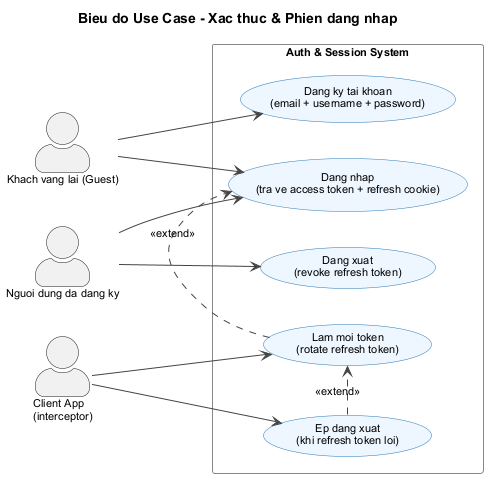
\includegraphics[width=0.80\textwidth, keepaspectratio]{UC-01-Auth.png}
  \caption{Hình 2.1: Biểu đồ Use Case — Nhóm Xác thực \& Phiên đăng nhập}
  \label{fig:uc01}
\end{figure}

\begin{figure}[H]
  \centering
  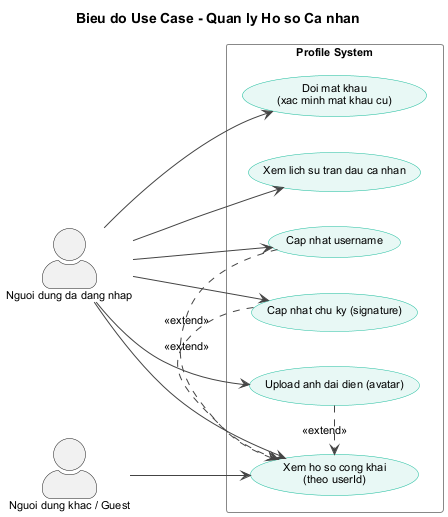
\includegraphics[width=0.80\textwidth, keepaspectratio]{UC-02-Profile.png}
  \caption{Hình 2.2: Biểu đồ Use Case — Nhóm Quản lý Hồ sơ cá nhân}
  \label{fig:uc02}
\end{figure}

% ----------------------------------------------------------
\subsection{Biểu đồ Use Case — Nhóm Phòng chơi}

Luồng tương tác quản lý phòng chơi (Hình~\ref{fig:uc03}) bao gồm tạo phòng, tham gia, đánh dấu
sẵn sàng và bắt đầu trận. System Actor chịu trách nhiệm tự động đóng phòng khi đến hạn \texttt{expiresAt}.

\begin{itemize}
  \item \texttt{Tham gia phòng} \textit{«include»} \texttt{Xem danh sách phòng}: phải tìm phòng
    trước khi tham gia.
  \item \texttt{Bắt đầu trận} \textit{«include»} \texttt{Đánh dấu sẵn sàng}: phải có ready flag.
  \item \texttt{Phòng hết hạn} \textit{«extend»} \texttt{Đóng phòng}: kích hoạt khi \texttt{expiresAt} đến.
\end{itemize}

\begin{figure}[H]
  \centering
  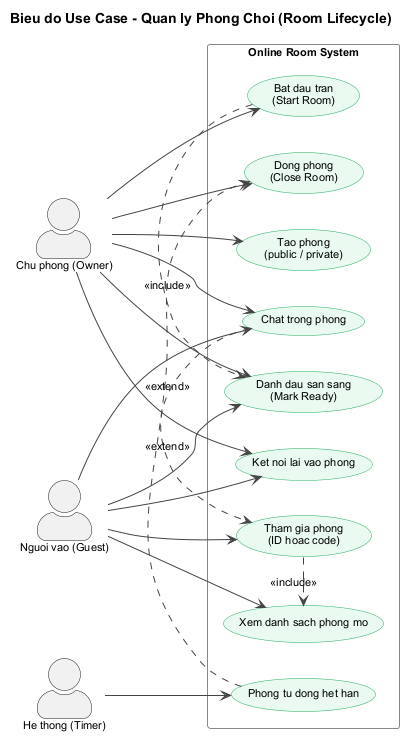
\includegraphics[width=\textwidth, height=0.55\textheight, keepaspectratio]{UC-06-RoomLifecycle.png}
  \caption{Hình 2.3: Biểu đồ Use Case — Quản lý Phòng chơi (Room Lifecycle)}
  \label{fig:uc03}
\end{figure}

% ----------------------------------------------------------
\subsection{Biểu đồ Use Case — Nhóm Xếp tàu \& Trận đấu}

\textbf{Giai đoạn xếp tàu} (Hình~\ref{fig:uc04}) mô tả quá trình từ lúc chủ phòng cấu hình bảng
đến khi cả hai người chơi xác nhận sẵn sàng. Owner và Player đều có thể xếp tàu thủ công (kéo
thả) hoặc ngẫu nhiên; thao tác xoay tàu là một phần của xếp thủ công. Khi hết \texttt{setupDeadlineAt},
System tự động xử lý người chưa sẵn sàng.

\begin{figure}[H]
  \centering
  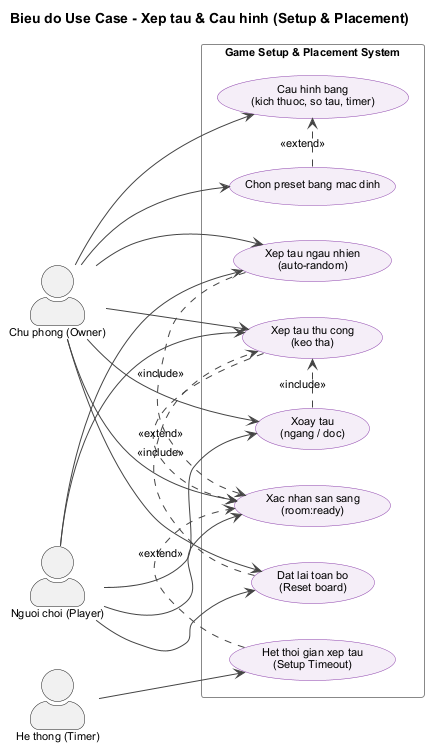
\includegraphics[width=\textwidth, height=0.55\textheight, keepaspectratio]{UC-04-GameSetup.png}
  \caption{Hình 2.4: Biểu đồ Use Case — Xếp tàu \& Cấu hình (Setup \& Placement)}
  \label{fig:uc04}
\end{figure}

\textbf{Giai đoạn trận đấu} (Hình~\ref{fig:uc05}) là cốt lõi của hệ thống: mô tả toàn bộ tương
tác trong một ván PvP, từ thực hiện nước đi, nhận phản hồi tức thì, đến khi xác định kết quả và
cập nhật Elo. System Timer đảm bảo tính công bằng bằng cách tự động chuyển lượt khi \texttt{turnDeadlineAt} hết.

\begin{figure}[H]
  \centering
  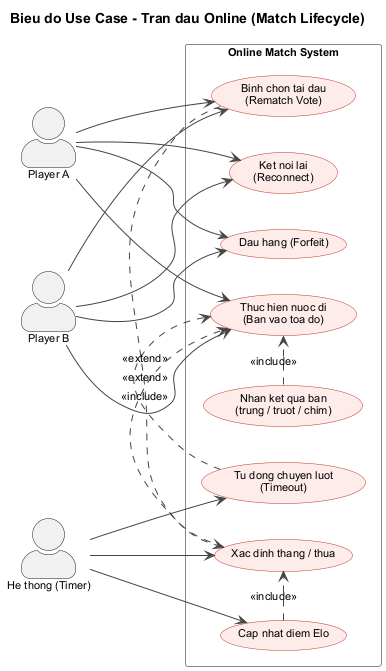
\includegraphics[width=\textwidth, height=0.55\textheight, keepaspectratio]{UC-07-OnlineMatch.png}
  \caption{Hình 2.5: Biểu đồ Use Case — Trận đấu Online (Match Lifecycle)}
  \label{fig:uc05}
\end{figure}

% ----------------------------------------------------------
\subsection{Biểu đồ Use Case — Nhóm Khán giả}

Khán giả (Hình~\ref{fig:uc06}) tham gia theo dõi trận đấu theo thời gian thực mà không can thiệp
vào diễn biến. Thông tin vị trí tàu bị ẩn hoàn toàn qua \texttt{SpectatorMatchSnapshot}. Kênh
chat riêng \texttt{room:roomId:spectators} tách biệt với kênh người chơi.

\begin{figure}[H]
  \centering
  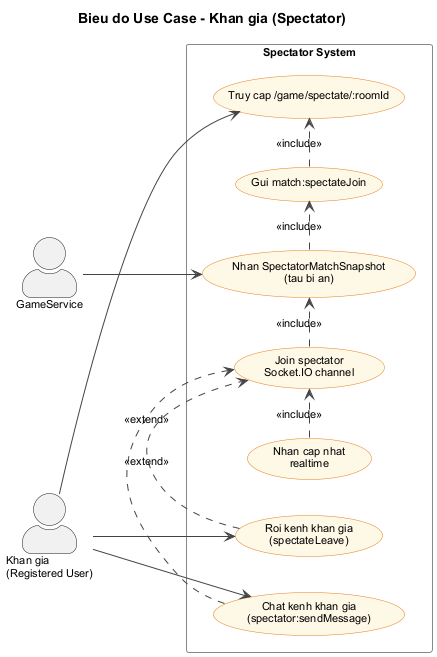
\includegraphics[width=0.85\textwidth, keepaspectratio]{UC-Spectator.png}
  \caption{Hình 2.6: Biểu đồ Use Case — Khán giả (Spectator)}
  \label{fig:uc06}
\end{figure}

% ----------------------------------------------------------
\subsection{Biểu đồ Use Case — Nhóm Cộng đồng}

Nhóm Cộng đồng (Hình~\ref{fig:uc07}) bao gồm bảng xếp hạng Elo (công khai với cả Guest), lịch
sử trận đấu cá nhân, diễn đàn bài viết và hệ thống bình chọn. Đây là lớp ``mềm'' giúp gắn kết
người chơi với nền tảng.

\begin{figure}[H]
  \centering
  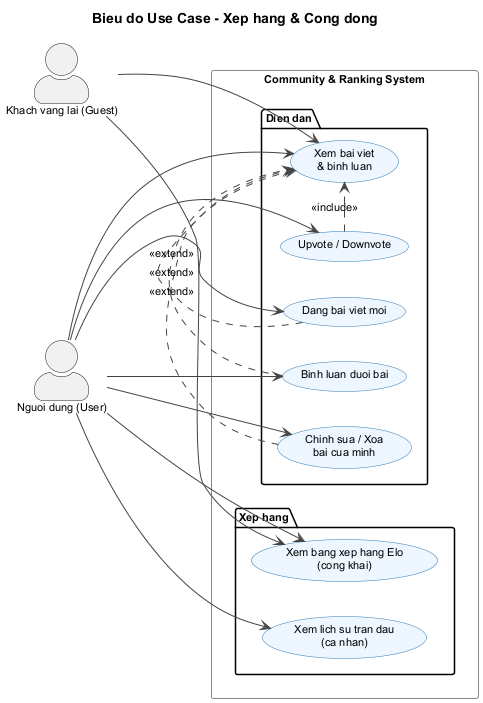
\includegraphics[width=0.90\textwidth, keepaspectratio]{UC-08-Community.png}
  \caption{Hình 2.7: Biểu đồ Use Case — Xếp hạng \& Cộng đồng}
  \label{fig:uc07}
\end{figure}

% ----------------------------------------------------------
\subsection{Biểu đồ Use Case — Nhóm Bot (Offline)}

Chế độ Bot (Hình~\ref{fig:uc08}) cho phép người chơi luyện tập mà không cần kết nối WebSocket
game. Toàn bộ logic xử lý phía client. Bot mức \textit{Hard} sử dụng thuật toán Hunt \& Target.
Kết quả không ảnh hưởng đến điểm Elo.

\begin{figure}[H]
  \centering
  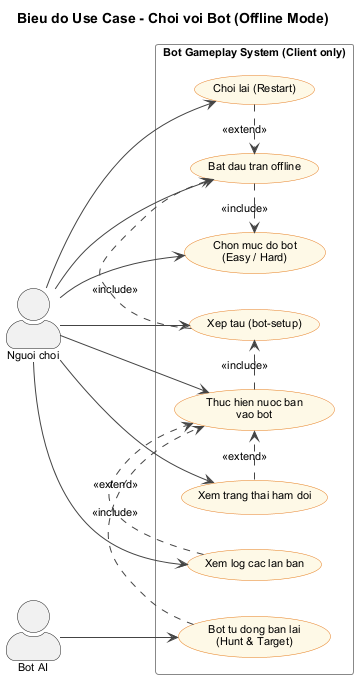
\includegraphics[width=0.85\textwidth, keepaspectratio]{UC-05-BotGameplay.png}
  \caption{Hình 2.8: Biểu đồ Use Case — Chơi với Bot (Offline Mode)}
  \label{fig:uc08}
\end{figure}

\end{document}
